\chapter{Experiência do Usuário}
\label{cap-exp-user}

Este trabalho visa contribuir diretamente com um software livre, tratando a evolução do mesmo. Dessa forma, neste capítulo, apresentamos os principais conceitos relacionados com esse tipo de software, passando pelas definições básicas, processos de desenvolvimento e os padrões para se contribuir com um projeto de software livre. Complementarmente, discutimos o que é evolução de software, tratando as Leis de Lehman e como está apresentada na literatura os estudos sobre a evolução de projeto de software livre.

%-------------------------------------------------------------------------------


%-------------------------------------------------------------------------------

\section{Requisitos Não-Funcionais}

\section{Usabilidade}

\subsection{Terminologias}
\label{sec-terminologias}

% No TCC 2, talvez, terminologia deve ser um capítulo inicial do trabalho.

O termo usabilidade de modo geral pode ser escrito como a facilidade com a qual
um equipamento ou programa pode ser usado. Esse termo dentro da computação foi
diversas vezes refinado como nas ISO 9126, 12119, 9241, 14598 e, por fim, na ISO
25010, que define como uma medida pela qual um produto pode ser usado por
usuários específicos para alcançar metas específicas com eficácia, eficiência e
satisfação em um contexto específico de uso~\cite{iso25010}.
%TODO: colocar referência da ISO.

%
A usabilidade não é uma qualidade intrínseca de um sistema, é dependente de um
acordo entre as características de sua interface e as características de seus
usuários na busca de determinados objetivos e situação de uso~\cite{cybis2010}.

%
Por esse motivo uma interface que pode ser considerada satisfatória para
determinado grupo de usuários pode ser inviabilizada por outros, como usuários
experientes \textit{versus} novatos, além de uma percepção diferente dependendo
do ambiente onde esse sistema se encontra, um computador lento \textit{versus}
computador rápido.
%
Dessa forma, podemos definir que a usabilidade é um acordo entre interface,
usuário, tarefa e ambiente. Baseado nesta definição é que pautaremos nossas
discussões e estudos de caso neste trabalho.

%
A necessidade de se garantir que sistemas e dispositivos estejam
adaptados à maneira como o usuário pensa, comporta-se e trabalha, entra o
conceito de ergonomia.
%
Tal conceito surgiu logo após a II Guerra Mundial, como consequência do trabalho
interdisciplinar realizado por diversos profissionais, tais como engenheiros,
fisiologistas e psicólogos, durante a guerra~\cite{lida2005}.

%
Há algumas definições formais para o termo ``ergonomia'', de acordo com a
\textit{Ergonomics Society}, a Associação Brasileira de Ergonomia e a 
\textit{International Ergonomics Association}.
%
Para este trabalho, adotamos a definição da Associação Brasileira de Ergonomia,
que a conceitua como o estudo das interações das pessoas com a tecnologia, a
organização e o ambiente, objetivando intervenções e projetos que visem
melhorar, de forma integrada e não-dissociada, a segurança, o conforto, o
bem-estar e a eficácia das atividades humanas \cite{abergo2013}.
%TODO: referência para o texto da ABE.

%
Neste contexto, a questão que norteia este trabalho é como pode-se avaliar,
entender, verificar, observar a interface de uma aplicação em determinado
contexto ou sistema?
%
Para respondermos essa questão, mapeamos as definições de alguns especialistas
em usabilidade e ergonomia, que estabeleceram critérios, regras e princípios
para nortear essa necessidade.

\begin{itemize}
\item Jakob Nielsen, em seu livro \textit{Usability Engineering} , propõe um
conjunto de dez heurísticas de usabilidade~\cite{nielsen1994}:

    \begin{itemize} 

    \item Viabilidade do estado do sistema;

    \item Mapeamento entre o sistema e o mundo realizada;

    \item Liberdade e controle ao usuário;

    \item Consistência e padrões;

    \item Prevenção de erros;

    \item Reconhecer em vez de relembrar;

    \item Flexibilidade e eficiência de uso;

    \item Design estético e minimalista;

    \item Suporte para o usuário reconhecer, diagnosticar e recuperar erros;

    \item Ajuda e documentação.

    \end{itemize}

\item Ben Shneiderman, em seu livro \textit{Designing The User Interface},
propõe, o que ele denominou de ``oito regras de ouro''~\cite{shneiderman2003}

    \begin{itemize} 

    \item Perseguir a consistência;

    \item Fornecer atalhos;

    \item Fornecer feedback informativos;

    \item Marcar o final dos diálogos;

    \item Fornecer prevenção e manipulação simples de erros;

    \item Permitir o cancelamento das ações;

    \item Fornecer controle e iniciativa ao usuário;

    \item Reduzir a carga de memória de trabalho.

    \end{itemize}

\item Christian Bastien e Dominique Scapin definiram 8 critérios ergonômicos~\cite{bastien1993}

    \begin{itemize}

    \item Condução;

    \item Carga de trabalho;

    \item Controle;

    \item Adaptabilidade;

    \item Gestão de erros;

    \item Coerência;

    \item Significado dos códigos;

    \item Denominações e Compatibilidade.

    \end{itemize}

\end{itemize}

Portanto, baseado nas heurísticas e critérios listados acima,  Walter Cybis, no
livro Ergonomia e Usabilidade, propôs uma tabela que relaciona todas essas
definições, conforme apresentado na Tabela \ref{tabela-walter-cybis}~\cite{cybis2010}.

%
\begin{table}[h]
\begin{tabular}{|l|l|}
\hline
Condução                               & \begin{tabular}[c]{@{}c@{}}Qualidade da ajuda e da documentação\\ Adequação ao aprendizado\\ Apresentação do estado do sistema\\ Convite\\ Agrupamento e distinção por localização\\ Agrupamento e distinção por formato\\ Feedback imediato\end{tabular} \\ \hline
Carga de trabalho                      & \begin{tabular}[c]{@{}c@{}}Legibilidade\\ Brevidade das entradas individuais\\ Concisão das apresentações individuais\\ Ações mínimas\\ Densidade informacional\\ Design minimalista e estético\end{tabular}                                              \\ \hline
Controle                               & \begin{tabular}[c]{@{}c@{}}Ações explícitas\\ Controle do usuário\end{tabular}                                                                                                                                                                            \\ \hline
Adaptabilidade                         & \begin{tabular}[c]{@{}c@{}}Flexibilidade\\ Personalização\\ Consideração da experiência do usuário\end{tabular}                                                                                                                                           \\ \hline
Gestão de erros                        & \begin{tabular}[c]{@{}c@{}}Proteção de erros\\ Tolerância aos erros\\ Qualidade das mensagens de erro\\ Correção de erros\end{tabular}                                                                                                                    \\ \hline
Coerência                              & \begin{tabular}[c]{@{}c@{}}Homogeneidade interna a uma aplicação\\ Homogeneidade externa a plataforma\end{tabular}                                                                                                                                        \\ \hline
Significado dos códigos e denominações & Interface clara                                                                                                                                                                                                                                           \\ \hline
Compatibilidade                        & \begin{tabular}[c]{@{}c@{}}Compatibilidade com o usuário\\ Compatibilidade com a tarefa dos usuários\\ Compatibilidade com a cultura dos usuários\end{tabular}                                                                                            \\ \hline
\end{tabular}
\caption{Conjunto integrador de critérios, princípios, regras e heurísticas de ergonomia}	
\label{tabela-walter-cybis}
\end{table}

\subsection{Técnicas de Usabilidade Ágeis}
\label{técnicas-usabilidade-ageis}


Técnicas de usabilidade e desenvolvimento ágil têm muito em comum, principalmente o fato de que, muitas vezes, estão envolvidos no desenvolvimento do mesmo software. Apesar disso, tem havido pouca investigação ou discussão sobre a forma como os dois processos trabalham em conjunto e os resultados dessa parceria. ~\cite{ferreira2007}.

%
Para tanto realizou-se uma revisão sistemática. A revisão sistemática é uma forma de síntese das informações disponíveis em dado momento, sobre um
problema específico, de forma objetiva e reproduzível, por meio de método científico. Ela tem como princípios gerais a exaustão na busca dos estudos analisados, a seleção justificada dos estudos por critérios de inclusão e exclusão explícitos e a avaliação da qualidade metodológica, bem
como a quantificação do efeito dos tratamentos por meio de técnicas estatísticas \cite{de2000psiquiatria}.

O Objetivo da revisão sistemática era levantar as técnicas de usabilidade em projetos ágeis aplicadas no desenvolvimento de software livre. A busca foi realizada nas bibliotecas digitais Google Academic e Springer Link que possuem máquinas de busca com bom funcionamento e abrangência, além das bases de teses e dissertações da UnB e USP. Como resultado do trabalho levantou-se uma lista de técnicas e foram selecionadas 5 das que mais poderiam ser facilmente aplicadas em projetos de software livre e evidenciadas abaixo.

\begin{enumerate}
%
\item Santos e Kon (\citeyear{santoskon2009}) propõe a aplicação do próprio processo de DCU (Design Centrado no Usuário) para levantamento dos usuários e do contexto de uso da metodologia. Os usuários do processo são membros de equipes de software livre, que desejam inserir práticas de usabilidade no processo de desenvolvimento. O contexto de uso são sistemas distribuídos geograficamente, com pessoas trabalhando colaborativamente. Os métodos podem ser aplicados tanto para o início de novos projetos, que tenham como usuários, pessoas não acostumadas a sistemas livres ou mesmo para a melhoria de sistemas existentes, com respeito à usabilidade.

%
\item Já Lee, Judge e McCrickard (\citeyear{lee2011}) defendem a aplicação de definição de histórias de usuário de usabilidade dirigidas pela decisão do responsável por design realizando a prototipação dessas histórias e depois sendo validadas através de testes de usabilidade conforme Figura \ref{fig:figuraCDR}.

\begin{figure}[H]
  \begin{center}
    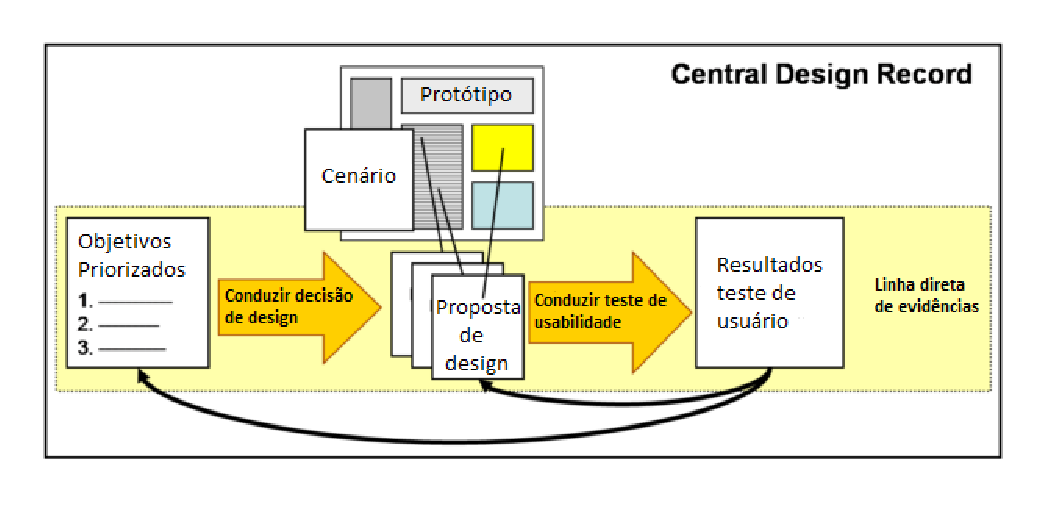
\includegraphics[width=0.5\textwidth]{figuras/figuraCDRBR.eps}
    \caption{Ciclo de atividades de usabilidade}
    \label{fig:figuraCDR}
  \end{center}
\end{figure}

%
\item As atividades de usabilidade seguem o modelo de ciclo de vida das outras atividades dentro do desenvolvimento ágil com a diferença que o ciclo de usabilidade tem sua iteração primeiro que as outras atividades de desenvolvimento conforme Figura \ref{fig:figuraCDR2}:

\begin{figure}[H]
  \begin{center}
    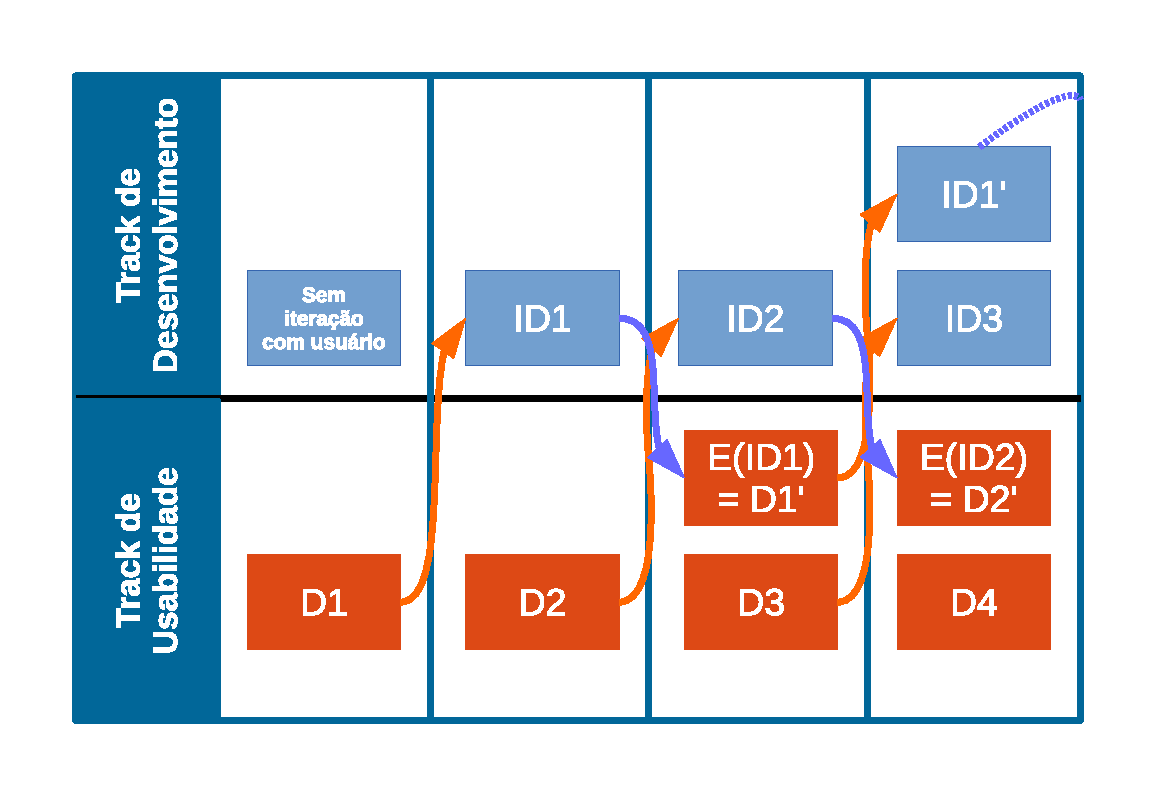
\includegraphics[width=0.5\textwidth]{figuras/FiguraTraducao1Color.eps}
    \caption{Ciclo das tarefas de usabilidade x desenvolvimento}
    \label{fig:figuraCDR2}
  \end{center}
\end{figure}

%
\item Santos (\citeyear{santos2012}) em uma nova pesquisa aplicada propôs a aplicação das técnicas de usabilidade de acordo com as fases do DCU, conforme a descrição das técnicas de usabilidade das comunidades de métodos ágeis e de software livre. Para a fase do DCU Criar soluções de design, não foram identificadas propostas de adaptações, sendo portanto, descritas propostas para as fases: Identificar necessidades para design centrado em humano, Especificar contexto de uso, Especificar requisitos e Avaliar Designs conforme tabela \ref{tabela-usabilidade-sl1}.

\begin{table}[h]
\begin{tabular}{|l|l|}
\hline
\multicolumn{2}{|c|}{\textbf{Práticas de usabilidade para Software Livre}}                                                                                                                                                                          \\ \hline
\textbf{Fases DCU}                                                                                 & \textbf{Práticas de Usabilidade}                                                                                                 \\ \hline
\begin{tabular}[c]{@{}c@{}}Identificar necessidades para \\ design centrado em humano\end{tabular} & \begin{tabular}[c]{@{}c@{}}Equipe-Núcleo como Donos do Produto\\ Caminhos Completos\\ Especialista-generalista\end{tabular}      \\ \hline
Especificar contexto de uso                                                                        & Pouco design antecipado e distribuído                                                                                            \\ \hline
Especificar Requisitos                                                                             & Definir metas de usabilidade automáticas                                                                                         \\ \hline
Avaliar designs                                                                                    & \begin{tabular}[c]{@{}c@{}}RITE (Rapid Iterative Testing and Evaluation)  \\ para desenvolvedores de software livre\end{tabular} \\ \hline
\end{tabular}
\caption{Práticas de usabilidade no contexto de Software Livre}	
\label{tabela-usabilidade-sl1}
\end{table}

%
\item Moreno e Yagüe (\citeyear{moreno2012}) trás em seu trabalho a inserção da usabilidade por meio da criação de User Stories de usabilidade que denominam de \textit{Usability Stories}. Tendo que especificar os recursos funcionais de usabilidade que serão utilizados no projeto, o artigo trás um tabela que é necessária para definir as características dessa funcionalidade.

\begin{table}[H]
\begin{tabular}{|l|l|}
\hline
Status do Sistema                                                      & Para informar os usuários sobre a situação interna do sistema                                                                                                                                                \\ \hline
Aviso                                                                  & \begin{tabular}[c]{@{}c@{}}Para informar os usuários de qualquer ação com consequências\\  importantes\end{tabular}                                                                                          \\ \hline
Longa ação Feedback                                                    & \begin{tabular}[c]{@{}c@{}}Para informar aos usuários que o sistema está processando\\  uma ação que vai demorar algum tempo para completar\end{tabular}            \\ \hline
Desfazer global                                                        & Para desfazer as ações do sistema em vários níveis                                                                                                                                                           \\ \hline
Abortar Operação                                                       & Para cancelar a execução de uma ação ou toda a aplicação                                                                                                                                                     \\ \hline
Abortar comando                                                        & Para cancelar a execução de uma tarefa em andamento                                                                                                                                                          \\ \hline
Voltar                                                                 & \begin{tabular}[c]{@{}c@{}}Para voltar a um estado particular em uma sequência de \\ execução de comando\end{tabular}                                                                                        \\ \hline
\begin{tabular}[c]{@{}c@{}}Entrada de texto\\ estruturada\end{tabular} & \begin{tabular}[c]{@{}c@{}}Para ajudar a prevenir o usuário de cometer erros de \\ entrada de dados\end{tabular}                                                                                             \\ \hline
\begin{tabular}[c]{@{}c@{}}Execução\\ Passo-a-Passo\end{tabular}       & \begin{tabular}[c]{@{}c@{}}Para ajudar os usuários a realizar tarefas que requerem \\ diferentes passos com a entrada do usuário e tal entrada correta\end{tabular} \\ \hline
Preferências                                                           & \begin{tabular}[c]{@{}c@{}}Para gravar as opções de cada usuário para usar as \\ funções do sistema\end{tabular}                                                                                             \\ \hline
Favoritos                                                              & Para gravar determinados locais de interesse para o usuário                                                                                                                                                  \\ \hline
Ajuda Multinível                                                       & Para fornecer diferentes níveis de ajuda para usuários diferentes                                                                                                                                            \\ \hline
\end{tabular}
\caption{Mecanismos de usabilidade}
\label{tabela-mec-usabilidade}
\end{table}

Associado a essas características é definido três maneiras pelas quais a incorporação de usabilidade influencia as histórias de usuário.
\begin{enumerate}
\item A adição de novas histórias para representar requisitos diretamente derivados usabilidade.
\item Adição ou modificação de tarefas em histórias de usuários existentes. Isto significa que algumas ações decorrentes de limitações de usabilidade devem ser realizadas por um usuário existente na história. Esta tarefa pode ser tão simples ou detalhados, conforme necessário.
\item Adição ou modificação de critérios de aceitação. Estes critérios de aceitação aparecem porque a funcionalidade da história de usuário precisa incluir algumas ações específicas para modificar o ambiente operacional.
\end{enumerate}

Com isso os autores realizaram um mapeamento entre os mecanismos de usabilidade e as ações a serem tomadas finalizando a proposta de como a usabilidade deve ser abordada por equipes ágeis.

\begin{table}[H]
\begin{tabular}{|l|l|l|l|l|l|l|}
\hline
                                                                       & \begin{tabular}[c]{@{}c@{}}Nova\\ Tarefa\end{tabular} & \begin{tabular}[c]{@{}c@{}}Modificar\\ Tarefa\end{tabular} & \begin{tabular}[c]{@{}c@{}}Novo\\ Critério de\\Aceitação\end{tabular} & \begin{tabular}[c]{@{}c@{}}Modificar\\ Critério de\\Aceitação\end{tabular} & \begin{tabular}[c]{@{}c@{}}Nova\\ História de \\ Usabilidade\end{tabular} & \begin{tabular}[c]{@{}c@{}}Nova\\ História\\ de Usuário\end{tabular} \\ \hline
Status do Sistema                                                      &                                                       & X                                                          & X                                                                      & X                                                                           & X                                                                                                                                                           &                                                                      \\ \hline
Aviso                                                                  & X                                                     &                                                            & X                                                                      & X                                                                           & X                                                                                                                                                           &                                                                      \\ \hline
Longa ação                                                             &                                                       & X                                                          & X                                                                      &                                                                             &                                                                                                                                                             & X                                                                    \\ \hline
Abortar Operação                                                       &                                                       & X                                                          & X                                                                      &                                                                             &                                                                                                                                                             &                                                                      \\ \hline
Abortar comando                                                        & X                                                     & X                                                          & X                                                                      &                                                                             &                                                                                                                                                             &                                                                      \\ \hline
Voltar                                                                 & X                                                     & X                                                          & X                                                                      &                                                                             &                                                                                                                                                             &                                                                      \\ \hline
\begin{tabular}[c]{@{}c@{}}Entrada de texto\\ estruturada\end{tabular} &                                                       & X                                                          & X                                                                      &                                                                             &                                                                                                                                                             &                                                                      \\ \hline
\begin{tabular}[c]{@{}c@{}}Execução\\ Passo-a-Passo\end{tabular}       & X                                                     &                                                            & X                                                                      & X                                                                           &                                                                                                                                                             &                                                                      \\ \hline
Preferências                                                           &                                                       &                                                            &                                                                        &                                                                             &                                                                                                                                                             & X                                                                    \\ \hline
Favoritos                                                              &                                                       & X                                                          & X                                                                      &                                                                             & X                                                                                                                                                           &                                                                      \\ \hline
Ajuda Multinível                                                       &                                                       & X                                                          & X                                                                      &                                                                             & X                                                                                                                                                           &                                                                      \\ \hline
\end{tabular}
\caption{Mapeamento entre os mecanismos de usabilidade e ações}
\label{tabela-map}
\end{table}
\end{enumerate}

%
O levantamento de técnicas de usabilidade da comunidade de métodos ágeis, técnicas
de usabilidade ágil, e das técnicas de usabilidade da comunidade de software livre, foi
realizado com o objetivo de refletir como técnicas de usabilidade poderiam ser aplicadas
em comunidades de software livre. E essa lista possibilitou uma escolha da técnica que melhor se adéqua ao estudo de casa de acordo com as características de cada uma encontrada na revisão sistemática. O trabalho completo da revisão sistemática pode ser encontrado na seção \ref{ap-revisao-sistematica} no apêndice do TCC.

\subsection{Usabilidade em Software Livre}
\label{usabilidade-sl}
%
Para aplicação em ambientes distribuídos, abertos e colaborativos, como em comunidades de software livre, implica-se uma adaptação em métodos de usabilidade. Isso ocorre porque em comunidades de desenvolvimento de software livre, não se pode garantir a existência de um indivíduo especialista em usabilidade ou de uma equipe dedicada a essas atividades. A distância física de membros que contribuem com o projeto também dificulta a utilização de métodos de usabilidade que dependem de comunicação face a face. Mesmo assim, a usabilidade deve ainda ser considerada, afinal ela é muito importante para a criação de um sistema de qualidade, em qualquer ambiente.

%
A usabilidade deve fazer parte do desenvolvimento, não apenas em busca de produtos usáveis, mas também de práticas usáveis e de modo a envolver todos os membros de uma equipe considerando o contexto em que as práticas serão aplicadas. Dessa forma, não se tem uma equipe de acordo com os valores de métodos ágeis e de métodos de usabilidade se apenas alguns se preocupam em atender as necessidades dos usuários típicos e clientes, pois todos os membros precisam entender a importância de atendê-las.
~\cite{santos2012}

%
Ana Paula Oliveira dos Santos , em sua dissertação de mestrado ~\cite{santos2012}, propôs práticas de usabilidade para a comunidade de software livre através da associação das fases do DCU(Design Centrado no Usuário) com as técnicas de usabilidade da comunidade ágil conforme a tabela \ref{tabela-usabilidade-sl}.

\begin{table}[h]
\begin{tabular}{|l|l|}
\hline
\multicolumn{2}{|c|}{\textbf{Práticas de usabilidade para Software Livre}}                                                                                                                                                                          \\ \hline
\textbf{Fases DCU}                                                                                 & \textbf{Práticas de Usabilidade}                                                                                                 \\ \hline
\begin{tabular}[c]{@{}c@{}}Identificar necessidades para \\ design centrado em humano\end{tabular} & \begin{tabular}[c]{@{}c@{}}Equipe-Núcleo como Donos do Produto\\ Caminhos Completos\\ Especialista-generalista\end{tabular}      \\ \hline
Especificar contexto de uso                                                                        & Pouco design antecipado e distribuído                                                                                            \\ \hline
Especificar Requisitos                                                                             & Definir metas de usabilidade automáticas                                                                                         \\ \hline
Avaliar designs                                                                                    & \begin{tabular}[c]{@{}c@{}}RITE (Rapid Iterative Testing and Evaluation)  \\ para desenvolvedores de software livre\end{tabular} \\ \hline
\end{tabular}
\caption{Práticas de usabilidade no contexto de Software Livre}	
\label{tabela-usabilidade-sl}
\end{table}

As práticas são descritas apresentando um contexto, um problema e uma solução visando a adequação a comunidades de software livre. Cada fase do DCU tem como objetivo: 

\begin{description}
\item[Identificar necessidades para design centrado em humano] Trazer o DCU para dentro da equipe-núcleo do projeto, tendo um responsável para assumir o papel de Proprietário do Produto,além da equipe-núcleo realizar o levantamento dos usuários, necessidades e o contexto do sistema e assumir o ciclo completo de DCU sem paralelismo com uma equipe externa de usabilidade;
\item[Especificar contexto de uso] Levar a equipe-núcleo a responsabilidade de especificar as práticas de usabilidade a serem utilizadas no contexto de uso do sistema;
\item[Especificar requisitos] Realizar a escrita de testes de aceitação automáticos baseados em BDD (\textit{Behavior Driven Development});
\item[Avaliar designs] Aplicação do método RITE (Rapid Iterative Testing and Evaluation) pela equipe-núcleo do projeto, sem necessidade de laboratórios de usabilidade podendo ser substituído por um acompanhamento da utilização dos usuários de um pequeno conjunto de funcionalidades.
\end{description}

A descrição completa dessas práticas pode ser encontrada na seção \ref{ap-praticas-usabilidade} no apêndice do TCC. Esta foi retirada da tese de mestrado da Ana Paula Oliveira dos Santos ~\cite{santos2012} e removido os exemplos aplicados em projetos realizados em sua tese. 

%
Assumindo as práticas descritas ao estudo de caso Mezuro, o ciclo de vida e aplicação destas na comunidade de software livre serão seguidos dentro do projeto junto com a equipe de desenvolvimento, visando suprir as deficiências e problemas citados no capítulo \ref{cap-introducao}.

\subsection{Métodos de Avaliação}
\label{metodos-avaliacao}

Uma  vez que conceituamos as práticas de usabilidade ágeis e o que 
encontramos sobre usabilidade em projetos de software livre, nesta seção
detalharemos os métodos escolhidos para a avaliação da ergonomia das interfaces. Os métodos de avaliação trás um diagnóstico através de verificações e inspeções de aspectos ergonômicos das interfaces que possam ser um problema ao usuário durante sua interação com o sistema. Através desse diagnóstico é possível priorizar e classificar os problemas encontrados de acordo com o método escolhido.

\subsubsection{Avaliação heurísticas}
Uma avaliação heurística representa um julgamento de valor sobre as qualidades
ergonômicas das Interfaces Humano-Computador. Essa avaliação é realizada por
especialistas em ergonomia, com base em sua experiência e competência no
assunto~\cite{cybis2010}.

%
Para utilização de uma avaliação heurística serão definidos os graus de
severidade. A severidade do problema de usabilidade é uma combinação de três fatores:
\begin{itemize}
\item A frequência com que ocorre o problema: é comum ou raro?
\item O impacto do problema caso ocorra: Será que vai ser fácil ou difícil para os usuários a superar ?
\item A persistência do problema: É um problema que com o tempo os usuários possam superar, uma vez que sabe sobre ele ou os usuários repetidamente serão incomodados pelo problema ?
\end{itemize}

A escala de classificação seguinte de 0 a 4 pode ser usada para avaliar a severidade dos problemas de usabilidade:~\cite{nielsen1995severity}:

\begin{itemize}

    \item 0 = Não há consenso quanto a ser um problema de usabilidade

    \item 1 = Problema cosmético

    \item 2 = Problema menor
	
    \item 3 = Problema importante de usabilidade

    \item 4 = Catástrofe de usabilidade

\end{itemize}

A presentação dos resultados seguirá um modelo simples similar ao que é
utilizado em desenvolvimento ágil para documentação de defeitos, elencando o
problema, a possível solução e o grau de severidade.
%TODOS: contextualizar e linkar este final com o foi dito antes... está vago.

\subsubsection{Inspeções por listas de verificação}
As inspeções de ergonomia por meio de listas de verificação permitem que
profissionais, não necessariamente especialistas em ergonomia, identifiquem
problemas menores e repetitivos das interfaces.
%
Nesse tipo de técnica, ao contrário das avaliações heurísticas, são mais as
qualidades explicativas da ferramenta e menos os conhecimentos implícitos dos
avaliadores que determinam as possibilidades para a avaliação~\cite{cybis2010}.

%
Através das inspeções de ergonomia será possível suprir um deficit ocasionado
pela falta de experiência do avaliador dentro de determinados contextos do
sistema que este não esteja familiarizado.
%
A ISO 9241 fornece listas de verificação de ergonomia bem definidas, porém será
utilizado as listas do laboratório LabIUtil do projeto
ErgoList~\footnote{\url{http:labiutil.inf.ufsc.br/ergolist/check.htm}},
que fornece um serviço na Internet para aplicar aplicarmos uma avaliação
simplificada e objetiva (\textit{check-list}) e obtermos os resultados
imediatamente.
%
Com a aplicação da lista pode obter vantagens como obter conhecimentos
ergonômicos, reduzir a subjetividade normalmente associada a processos de
avaliação e sistematizar as avaliações se tratando de abrangência de componentes
a inspecionar.

Com a aplicação dos métodos de avaliação será obtido os relatórios com os diagnósticos da verificação e inspeção dos aspectos ergonômicos. Estes possibilitarão a classificação (de acordo com cada método) e a priorização dos problemas encontrados, fator fundamental para sustentar as práticas de usabilidade adotadas para a implementação no estudo de caso Mezuro descritas na seção \ref{usabilidade-sl}. Ter o controle dos problemas levantados e seus impactos na aplicação, irá auxiliar na tomada de decisão da equipe e deixará todos cientes do andamento da usabilidade no projeto e sua importância dentro do desenvolvimento. 

\section{Visualização de Software}

%importancia da visualização, geral
O progresso alcançado com sistemas de hardware possibilita que grandes quantidades de informações sejam armazenadas por sistemas computacionais. Aproximadamente um exabyte, quantidade equivalente a um milhão de terabytes, de dados é gerado a cada ano, das quais a maior parte está disponível na forma digital \cite{keim2002information}. Um dos fatores que contribuem para isso são o avanço das tecnologias da informação e das telecomunicações, além da diminuição dos custos dos dispositivos de armazenamento. Dados armazenados podem auxiliar no apoio aos mais diversos tipos de atividades como definição de políticas públicas, investigações científicas, estratégias de negócios, melhoria da qualidade de sistemas de software. Mas para que os dados possam ser aproveitados ao máximo, é necessário primeiro compreendê-los \cite{heer2012interactive}. referencia

A visualização fornece meios poderosos para a compreensão de grandes conjuntos de dados. Por meio de representações gráficas e interativas apoiadas por computador é possível mapear atributos ou características, relativos ao domínio observado, em propriedades visuais como posição, tamanho, forma e cor potencializa as habilidades sensoriais do ser humano para o entendimento, tomadas de decisão e interpretação de padrões, agrupamentos, tendências e discrepâncias. A partir de uma representação inicial, o usuario extrai observações e conclusões sobre os dados e interage diretamente com a visualização, moldando-a para atingir os objetivos de sua tarefa \cite{rafaelmessiasmartins2012}.

O estudo da visualização de informações pode ser dividida em duas grandes vertentes. A primeira é a visualização científica que trata de dados físicos ou geométricos, como o planeta Terra, o corpo humano e fenômenos da natureza. A segunda vertente está relacionada a informações não-físicas, como dados financeiros, coleçoes de documentos, código-fonte de sistemas de software, os quais podem se beneficiar de representações visuais \cite{rafaelmessiasmartins2012}. Porém, para esse tipo de informação é necessário aplicar técnicas de visualização, pois não há formas diretas para representá-las. %referenciar card et. al 1999

A visualização de informação é composta por dados de entrada, que consistem em grandes conjuntos de registros. Cada registro contem certo número de atributos ou dimensões. A quantidade de dimensões define a dimensionalidade do conjunto de dados, que pode ser bidimensional ou multidimensional. Conjuntos de dados multidimensionais exigem técnicas mais sofisticadas para sua representação, já que não podem ser mapeados diretamente nos espaços 2D ou 3D, ao contrário dos bidimensionais.

Plataformas de avaliação de qualidade baseadas em conjuntos de ferramentas, como é o caso do Mezuro, expõem o avaliador de qualidade a dezenas de valores numéricos relacionados as métricas calculadas. Sem uma apresentação especial, esses dados são de pouco valor, pois são numerosos e difíceis de avaliar. Muitas vezes as métricas não são correlacionadas e a formatação da apresentação consiste apenas na aplicação de valores de referência.

Uma possibilidade para a solução desse problema é a exploração da visualização de software, uma sub-área da visualização de informações cujos objetivos são auxiliar a compreensão de software e melhorar a produtividade do seu processo de desenvolvimento utilizando visualização, já que essa sub-área gera representações visuais de diversos aspectos do software e de seu processo de desenvolvimento \cite{rafaelmessiasmartins2012}, como processos de análise e especificação de requisitos, design e arquitetura, implementação, manutenção e evolução de software.

A visualização de software é uma das ramificações da visualização de informação que mais cresce atualmente. A visualização de software é dividida em três categorias principais: estrutura, comportamento e evolução.
%tecnicas para visualização em geral: https://github.com/mbostock/d3/wiki/Gallery
\begin{itemize}
\item \textbf{Estrutura} é a categoria que representa as partes estáticas do sistema, ou seja, aquelas que podem ser computadas sem executá-lo como por exemplo o código-fonte, estrutura de dados do programa, o grafo de chamadas estático, e a organização do programa em módulos.

A maioria das ferramentas, técnicas, propostas nessa categoria compartilham um mesmo modelo conceitual: a geração de um grafo, onde vértices representam entidades do programa, como arquivos ou classes, e arestas representam dependências como usos, chamadas, ou heranças.

%tecnicas de visualição dessa categoria, de acordo com Rafael Messias:
%codecity, treemap, HEB
%Grande parte das ferramentas propostas na categoria Estrutura compartilham um
%mesmo modelo conceitual: a geração de um grafo, onde vértices representam entidades
%do programa, como arquivos ou classes, e arestas representam dependências como usos ou
%heranças. A técnica Hierarchical Edge Bundles (HEB) (Holten, 2006), ilustrada na Figura
%3.3,  ́e utilizada para visualizar ao mesmo tempo duas informações do grafo: a estrutura
%hierárquica dos arquivos do código fonte e suas dependências, ou seja, as chamadas entre
%funções ou métodos.

\item \textbf{Comportamento} se refere a compreensão do que ocorre com o sistema durante seu tempo de execução, quais instruções são executadas e como seus estados mudam dado um conjunto de possíveis entradas. Entre as aplicações dessa categoria de visualização estão a análise de traces, que são registros de valores de variáveis em certos instantes, animação de algoritmos, depuração visual, e apoio visual a atividade de teste. 

%As técnicas dessa categoria NÃO são importantes para o Mezuro (pelo menos até agora)
\item \textbf{Evolução} representa as características modificadas ao longo do tempo em um sistema. Técnicas de visualização dessa categoria podem auxiliar analistas a verificarem quais as relações entre artefatos modificados e quais tendências dessas modificações. Analisar a evolução de um sistema pode ser tão ou mais importante que a análise de sua estrutura, já que manutenções, sejam elas corretivas, preventivas ou adaptativas representam grande parte do custo envolvido em um projeto, podendo chegar a até 80\% do total.
%técnicas presentes na categoria de evolução:
\end{itemize}

Como o Mezuro é uma plataforma de análise de código-fonte, ou seja, análise estática, a categoria de visualização de software comportamento, responsável por fornecer informações da execução do sistema, não será relevante para este trabalho, ao contrário das categorias estrutura e evolução.

Selecionar uma técnica de visualização mais relevante para um objetivo ou aplicação particular não é trivial, já que nenhuma técnica específica funciona bem para todos os casos ou problemas (Thomas e Cook, 2005).

%importancia visualização em softwares livres
%As vantagens proporcionadas pela visualização motivam a exploração dessa área do conhecimento em projetos de sofwares livres. Em projetos FOSS há diversas informações que podem ser utilizadas para compreender a qualidade do projeto desenvolvido. Porém a quantidade de informações e a própria natureza do código-fonte, como tratado na seção \ref{sec-proc-sl}, tornam essas informações pouco eficazes para auxiliar processos de melhoria.

Para alcançar as representações gráficas e todas as vantagens proporcionadas pela visualização de software, é necessário primeiro extrair as métricas de código-fonte e repositório.

\subsection{Métricas de Qualidade}

O processo de extração de métricas, muitas vezes, gera um grande volume de métricas, com valores predominantemente núméricos, que ainda são difíceis de analisar sem ferramentas apropriadas. O objetivo da visualização de informação aplicada a softwares, não apenas livres, é possibilitar que grandes quantidades de informações, as métricas extraídas, sejam analisadas objetivamente para compreensão de sua qualidade. Isso permite estabelecer um processo para apoiar as tarefas de avaliação, monitoramento e melhoria da qualidade.

%Motivação
Muitas vezes as avaliações de projetos FOSS são feitas informalmente, com a leitura de documentação e análise de opiniões de usuários anteriores, que nem sempre geram resultados confiáveis. Nesses projetos, muitos dados, tanto de processo como de produto, estão disponíveis publicamente. Exemplos desses dados são: código-fonte, históricos de evolução do repositório, conjunto de testes, relatório de erros, entre outros. Todas essas informações, se corretamente processadas, podem ser utilizadas para avaliar a qualidade de projetos. 

Métricas podem ser usadas para medir características e atributos definidos por modelos de qualidade de software voltados para a análise tanto do processo quanto do produto. Alguns modelos propostos especificamente para FOSS se baseiam em modelos tradicionais como o CMMI\footnote{Capability Maturity Model Integration}\cite{paulk1994capability} e a norma ISO 9126\cite{iso2003iec} mas incluem extensões que consideram especificamente aspectos importantes do desenvolvimento aberto. No entanto, a multiplicidade de indicadores de qualidade que podem ser extraídos de um projeto FOSS, considerando todas as suas diversas perspectivas (principalmente código, testes e repositório), cada um com suas próprias interpretações e valores de referência, torna complicada a realização de uma avaliação objetiva e direta. Abaixo se encontram as métricas disponibilizadas pelas ferramentas base utilizadas na plataforma Mezuro.

\graphicspath{{figuras/}}
\begin{figure}[H]
\centering
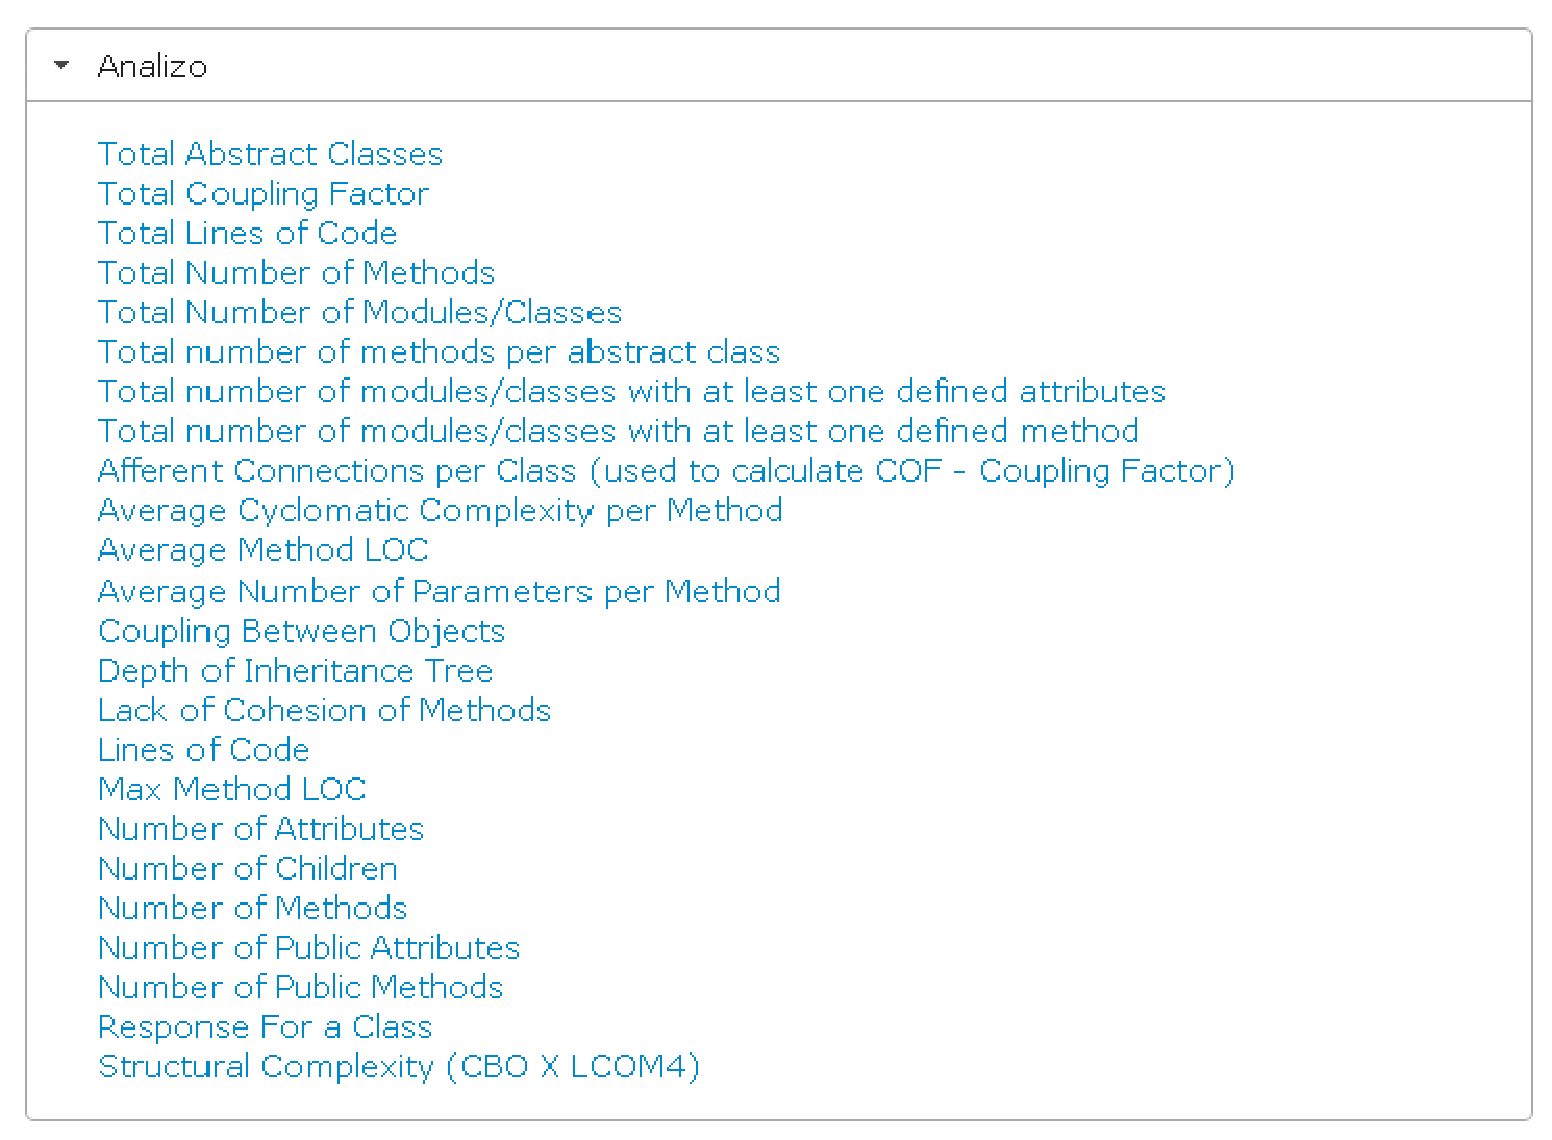
\includegraphics[width=0.8\textwidth]{analizo_bt}
\caption{Métricas fornecidas pela ferramenta base Analizo}
\label{fig-analizo_bt}
\end{figure}

O Analizo possui suporte nativo às linguagens C, C++ e Java, extraindo métricas de código-fonte (entre elas há mais de quinze métricas de módulos e sete métricas de projetos). Além dessas características, o Analizo também apoia a evolução de software já que permite a análise de diferentes versões do software em relação ao tempo .

\graphicspath{{figuras/}}
\begin{figure}[H]
\centering
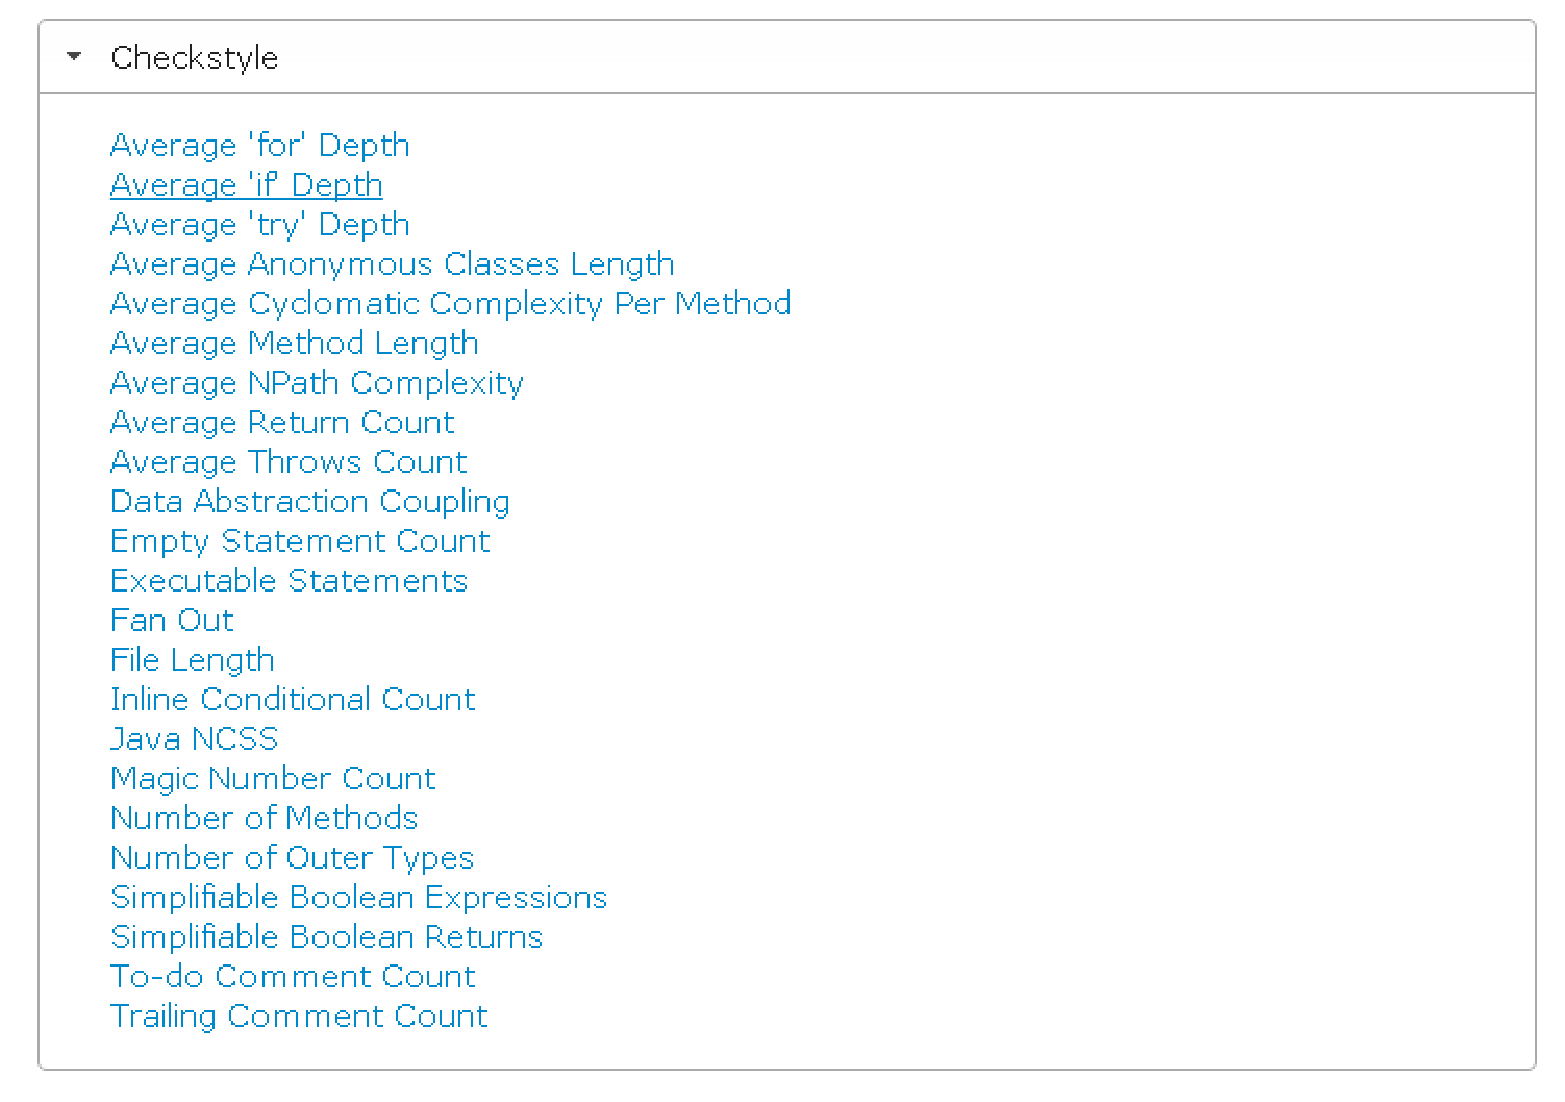
\includegraphics[width=0.8\textwidth]{checkstyle_bt}
\caption{Métricas fornecidas pela ferramenta base Checkstyle}
\label{fig-checkstyle_bt}
\end{figure}

O Checkstyle é uma ferramente de desenvolvimento que tem como principal objetivo auxiliar os desenvolvedores a seguirem um padrão de codificação. Assim como o Analizo, é através da extração de métricas de código-fonte Java que essa ferramenta visa alcançar o padrão de codificação pretendido.

\graphicspath{{figuras/}}
\begin{figure}[H]
\centering
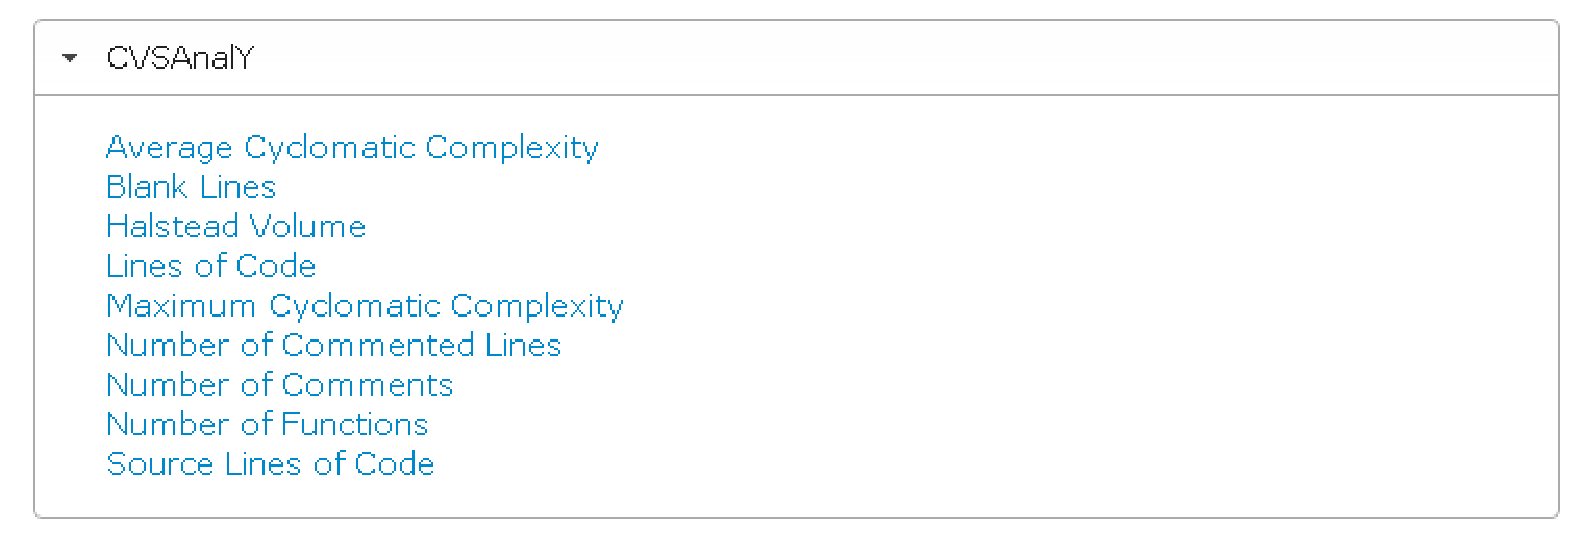
\includegraphics[width=0.8\textwidth]{cvsanaly_bt}
\caption{Métricas fornecidas pela ferramenta base CVS Analy}
\label{fig-cvsanaly_bt}
\end{figure}

%qual linguagem de suporte, realmente essas informações são verídicas?
Dentre os coletores de métricas utilizados no Mezuro, o último a ser adicionado foi o CVSAnaly, que apesar de não ampliar o suporte do Mezuro a novas linguagens, ele aumenta a variedade de métricas disponíveis já que muitas das métricas extraídas por essa ferramentas são complementares às métricas do Analizo e do Checkstyle.